\documentclass[12pt,A4]{article}
\usepackage{geometry}                % See geometry.pdf to learn the layout options. There are lots.
\geometry{letterpaper}                   % ... or a4paper or a5paper or ...
%\geometry{landscape}                % Activate for for rotated page geometry
\usepackage[parfill]{parskip}    % Activate to begin paragraphs with an empty line rather than an indent
\usepackage{graphicx}
\usepackage{amssymb}
\usepackage{multicol}
\usepackage{amsmath}
\usepackage{amsfonts}%to get the mathbb alphabet
\usepackage{epstopdf}
\usepackage{color}
\usepackage[square]{natbib}  %\usepackage[round]{natbib} to cite as (2)
\usepackage{subfigure}
\DeclareGraphicsRule{.tif}{png}{.png}{`convert #1 `dirname #1`/`basename #1 .tif`.png}

\title{ A report on Borehole tomography}
\author{\small $^{1}$Fasil Tesema  \\  \small {\color{black}$^{1}$Washera Geospace and Radar Science Laboratory (WaGRL)}\\\small  {\color{black}Bahir Dar University, College of Science,  Bahir Dar, Ethiopia }  \\ }%\\  \small {\color{black}$^{2}$Boston College, Institute for Scientific Research, Boston, USA }}
\date{December 2013}
\begin{document}
\maketitle

\begin{abstract}
We consider a borehole tomography within the framework of Bayesian statistical inversion. The objective is to study properties of the ground, for example for mining processes. In dealing with such a technique that is used to explore mine inside the Earth, transmitters will be located inside the Earth form one borehole and receivers from the other and at the surface of the ground. A wave on the way from transmitters to receivers experience intensity attenuation due to the composition of the Earth in attention. By measuring the attenuated intensity at the receivers one can estimate the unknown composition of the Earth using principle of inverse problem. This paper presents the idea of estimating the unknowns from the measurements obtained on the basis of Bayesian statistical inversion.


\end{abstract}

\section{Introduction}
Tomography is an inversion technique which is designed to analyze the structure, composition and spatial distribution of a certain physical parameter of an object by examining them with waves from many directions. The waves used to study the object can be electromagnetic or acoustic in origin. Depending on the structure of the object, these waves can be emitted, absorbed, transmitted, reflected, refracted or diffracted or a combination of these. Therefore, we speak of emission, reflection, transmission and diffraction tomography. In all cases, waves from many propagation and viewing directions results in better reconstruction of an object. 
Based on the propagation and viewing directions the imaging covers the mapping of one or more physical parameters across one or more planes.  \\

In combination with the electronic measurement setup, the processing of the collected information thus plays a crucial role in the production of the final image. Tomographic systems calculate the value of the respective physical parameter at all vertices of the grid that serves for the spatial encoding of the image (Menke,2012; Tarantola,2005). Some of imaging systems such as cameras, camcorders, or microscopes is the sensor that directly delivers the observed image. However, in tomography, the sensor performs indirect measurements of the image by detecting the radiation with which the object is examined. For each measurement, the emerging radiation is the sum of the contributions of the quantity to be reconstructed along the traversed path, each elementary contribution being either an elementary source of radiation or an elementary interaction between radiation and matter. It is mathematically equivalent to reconstruction of a two dimensional function from its line integrals. These set of line integrals, which defines the measurement equation constitutes the direct problem, linking the unknown quantities to the measurements. The image reconstruction will be done by solving this system of integral equations, i.e. the inverse problem.\\
Based on the wavelength of the wave and the property of the object, tomography can be divided in to two categories: ray tomography and diffraction tomography. If the object does not change over one wavelength, the wave propagation is almost along straight lines (rays). Thus, ray equation or geometrical optics is used for the formulation of wave propagation. When the wavelength is too long for geometrical approximation, diffraction concepts have to be accounted based on wave equation. 
\\\\
Borehole tomography uses seismic waves to analyze the structure and composition of the Earth. Transmitters will be located inside the Earth form one end and receivers from the other end and at the surface of the Earth. A wave on the way from transmitters to receivers experience intensity attenuation due to the composition and structure of the Earth in attention. The attenuated intensity that can be measured at the receivers is the indirect way to search for the compositions that let this attenuation happen. This type of indirect observations to get the unknown attenuation coefficients, which cannot be measured directly, is the basic idea of inversion in seismic tomography. \\
The intensities of the wave at the receptor and at the transmitter can be related as (Beer-Lambert law),
\begin{equation}
I=I_{o}\left[e^{-\int_{s} X(s)ds}\right].
\end{equation}
This equation can be written in the form of,
\begin{equation}
m_{j}=\int_{s}X(s)ds,
\end{equation}  
where $m_{j}=log(I_{o}/I)$ is the measurement at the $j^{th}$ receiver along the straight path $s$.
Using Riemann sum approximation the above equation can be written as
\begin{equation}
m_{j}=\sum_{k=1}^{n}\omega_{j,k}X_{k},\hspace{0.8cm}j=1,2,...,m
\end{equation}
where $\omega_{j,k}$ are the weight parameters along the straight path $s$, and $X_{k}$ are the attenuation coefficients in the grid. Here we assume the ray path $s$ is a straight line from the transmitter and receiver (a ray-cast assumption).

\section{Forward problem}
Forward problem is a prediction of the results of a measurement on the basis of some general principle or model (equation (1)) and a set of specific conditions relevant to the problem at hand. When numerically solving integral in (2), it is always reduced to a system of algebraic equations in (3). The measurements and the unknown attenuation coefficients in the grid can be put into a column vector $M$ and $X$ respectively. After this, the problem of the tomography may be written in the form of 
\begin{equation}
M=WX,
\end{equation}
where $M\in R^{m}$ is set of measurements, $W\in R^{m\times n}$ is a matrix with weighting parameters and $X\in R^{n}$ is the unknown coefficient matrix. However, in reality measurements are corrupted by noise.
\begin{equation}
M=WX +E,\hspace{0.8cm}E\thicksim N(0,\sigma^2I)
\end{equation}
where $E\in R^{m}$ is a noise vector that comes from for example instrument errors and assumed to be a zero mean Gaussian with unknown variance $\sigma ^{2}$. The above equation is usually referred as additive noise model. The main idea here is to estimate the attenuation coefficients $X$ from a given measurement data $M$ and the theory matrix $W$ based on the location of the transmitters and receivers. In this paper the estimation is presented from the Bayesian point of view, which is based on the probability theory and randomness assumption of all the unknown parameters. Moreover, the unknowns are considered to be stationary (the evolution of the parameters is not taken in to account).\\
By defining the attenuation coefficients in the grid ($N$ by $M$) with $n$ pixels and placing number of transmitters ($Tx$) and receivers ($Rx$) at a specified location (for example, see Figure 1) we can calculate the theory matrix $W$ and generate (simulate) the measurement ($M$) using equation (5). 
%The dimension of the theory matrix here will be $(Rx\times Tx)$ by $(N\times M)$ and the dimension of the measurement matrix ,which is equal to the number of rays from transmitter and receiver pairs, is $(Rx\times Tx)$ by $1$.
\begin{center}
\begin{figure}[h]
{\centering {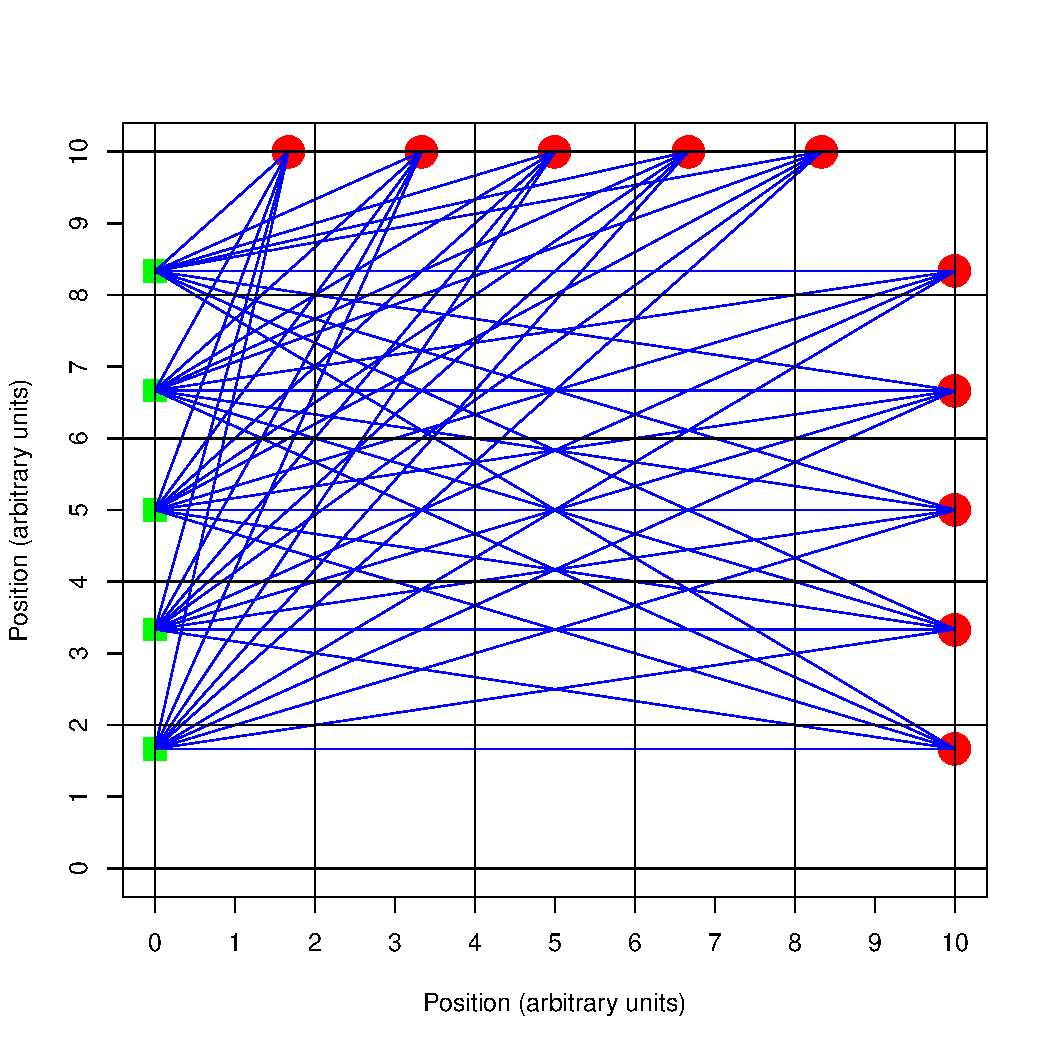
\includegraphics [scale=0.5] {fig1.pdf}}\par}
\caption{Positions of transmitters (green rectangles) and receivers (red circles) on a grid size of 5 by 5 (forward.m or forward.r).}
\end{figure}
\end{center}
\section{Inverse problem}
Once we have the measurement the main goal is to estimate the unknown attenuation coefficients in the grid based on statistical inversion. The statistical model to solve inverse problems consists of constructing the likelihood and the prior model. The likelihood model expresses the distribution of the measurement as if the unknown X and other parameters of the observation model is known and fixed. The prior model, which comprises all the information of the unknown prior to measurement, will be constructed on the basis of previous experience and our belief about the unknown.\\\\
If the noise in equation (5) does not depend on $X$, fixing $X=x$ doesn't change the distribution of $E$, then the probability distribution of the error given $x$, $\pi(e|x)$, is given by
\begin{equation}
\pi(e|x)=\pi(e)=\pi_{noise}(e).
\end{equation}
Since $X$ is fixed the only randomness in the measurements $M$ is due to $E$
\begin{equation}
\pi(m|x)=\pi_{noise}(M-WX).
\end{equation}
This shows that the randomness is translated by the model given in equation (5). 
The distribution of the noise is not fully determined, and depend on the unknown parameters $\theta$. Here in the above equation we claim as if the unknown parameters $\theta$ are known and fixed. The likelihood model is then
\begin{equation}
\pi(m|x,\theta)=\pi_{noise}(M-WX|\theta).
\end{equation}
As we already assumed the Gaussian white noise, the likelihood model takes the form
\begin{equation*}
\pi(m|x,\sigma^2)=C\hspace{0.2cm}exp\left(-\frac{1}{2\sigma^2}\parallel M-WX\parallel ^2\right)
\end{equation*}
\begin{equation}
\pi(m|x,\sigma^2)\propto\hspace{0.2cm}exp\left(-\frac{1}{2}( M-WX)^{T}(\sigma^2 I)^{-1} (M-WX)\right)
\end{equation}
%If we choose the prior a zero mean Gaussian process with a known co-variance $C$, we can define
%$$C^{-1}=L^{T}L,$$ 
If we assume the simple difference prior model, 
\begin{equation*}
LX+e'=0,\hspace{0.8cm}e'\thicksim N(0,\alpha^{2} I)
\end{equation*}
\begin{equation}
\pi(x)\propto exp\left(-\frac{1}{2\alpha^{2}}(LX)^{T}(LX)\right). 
\end{equation}
From Baye's formula,
\begin{equation}
\pi(x|m)=\frac{\pi(m|x)\pi(x)}{\pi(m)}.
\end{equation}
The likelihood distribution given in (9) and the above equation results in
\begin{equation}
\pi(x|m)\propto exp\left(-\frac{1}{2}\left[(LX)^{T}(\alpha^{2} I)^{-1}(LX)+( M-WX)^{T}(\sigma^2 I)^{-1} (M-WX)\right]\right).
\end{equation}
This general posterior distribution, which is the solution of the inverse problem, leads us to obtain several different estimates. The most widely used in inverse problem is the maximum posterior estimate, which is the same as conditional mean estimate in the Gaussian distribution. It can be put as
\begin{equation}
x_{map}= \left(L^{T}(\alpha^{2} I)^{-1}L+W^{T}(\sigma^2 I)^{-1} W\right)^{-1}W^{T}(\sigma^2 I)^{-1}M.
\end{equation}
However, in the case of classical inversion theory the solution of (6) is obtained by Tikhonov regularization. In Tikhonov regularization one minimizes the function
\begin{equation}
T(x)=\parallel M-WX\parallel ^2+ \beta^{-2}\parallel LX\parallel ^2,
\end{equation}
where $\beta=\alpha/\sigma$ and $L$ is a linear $l^{th}$ order difference matrix. The minimum of the above function, which is the Tikhonov regularized solution, is exactly the same as the map estimate in (13). But, in statistical inversion approach we do have a wide information to study the property of posterior covariance (Tarantola, 2005),
\begin{equation}
A= \left(L^{T}(\alpha^{2} I)^{-1}L+W^{T}(\sigma^2 I)^{-1} W\right)^{-1}
\end{equation}
From series of equations derived above (equation 4 to 13) one can infer some basic ideas in the inversion process. The first thing is to define a model which relates the unknown parameters and the measurement called observation (measurement) model. This model should include all the possible parameters that directly or indirectly affect our measurement. If there are parameters out of our interest we can marginalize in the process using probability theory. The second one is to have an appropriate prior model, by appropriate we mean all the information about our unknown should be included in the prior. The prior is the one to guide our estimation in the proper direction. If we have a weak prior our estimation will be far from our expectation. \\\\
As an example simulation of measurements from five transmitters and ten receivers using an assumed true model (an image of 625 pixels) was done as shown in Figure 2. From these measurements the MAP estimate is obtained by having number of pixels different from the one used to simulate the measurements (to avoid inverse crime). The prior model used for the inversion is a first order difference prior along the vertical and horizontal direction.
Since the number of measurements is less than the unknowns in Figure 2, the system is under-determined. This shows that depending on the grid size and or the number of transmitters and receivers we can have different systems and simulation results. In the next section we will discuss the estimation of our unknown by changing the number of transmitters and receivers and grid size.
\begin{center}
\begin{figure}[h]
{\centering {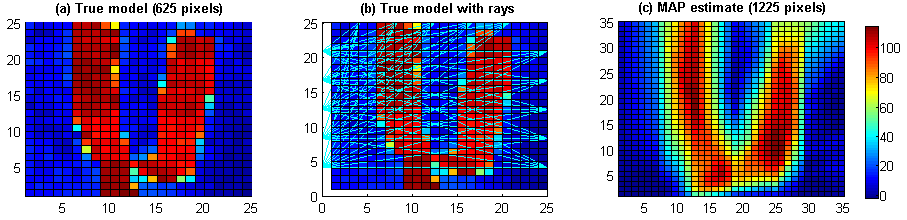
\includegraphics[scale=0.65]{fig2.png}}\par}
\caption{Estimation of the true model (625 pixels) using five transmitters and ten receivers with $\alpha^{2}=1.42$ . 50 measurements (b) used to estimate 1225 unknowns (c) (under-determined system)(final2.m).}
\end{figure}
\end{center}

\section{Transmitters, receivers and grids}
After defining the true model in (5) and setting the position of the transmitters and receivers, simulated measurement from each transmitter receiver pairs can be obtained as discussed in section 2. The idea is to estimate the unknown in the grid based on the inversion discussed in section 3. To see how the inversion is done we consider an image of $n$ pixels as a true model.

Here we assume the true model is an image of dimension (25 by 25 grid or 625 pixels), which is used to simulate the measurements. In addition, a first order difference Gaussian prior with known and fixed variance of the innovation $\alpha^{2}$ is used in the inversion. To get a better estimation of the unknown there should be many measurements in different direction or a small discretization step in the process. Based on the experimental setup shown in Figure 1 one can increase or decrease the number of transmitters and receivers in order to have many or few measurements respectively. If the number of measurements is greater than the number of pixels the system will be over-determined (Figure 3(c)). If the number of pixels is greater than the number of measurements the system is under-determined (Figure 3 (a)(b) and Figure 4). Comparing Figure 3 (a), (b) and (c) it can be noted that the values of each pixel approaches to the true model values. However, Figure 4 shows the estimation of the pixels values in the grid with different grid sizes (number of pixels). Figure 4 (a) is a finer resolution of the estimated values than (b) and (c). In general, having more pixels with fixed number of receivers and transmitters gives fine resolution of the reconstruction. Increasing the number of transmitters and receivers to improve the resolution is not practical and always possible due to the amount of survey needed (cost).
\begin{center}
\begin{figure}[h]
{\centering {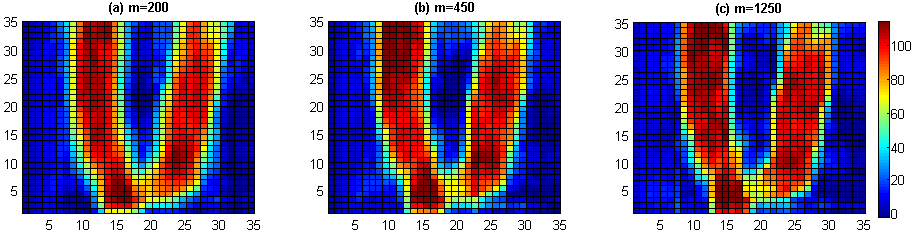
\includegraphics  [scale=0.65]{fig3.png}}\par}
\caption{Estimation using different measurements (different number of transmitters and receivers) with the same grid size 35 by 35 and $\alpha^{2}=1.42$ (fina12.m).}
\end{figure}
\end{center}

\begin{center}
\begin{figure}[h]
{\centering {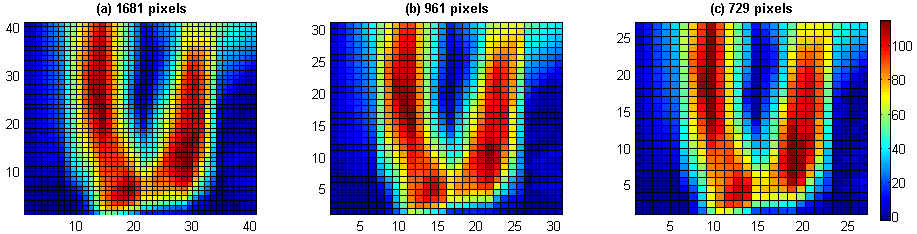
\includegraphics [scale=0.65]{fig4.png}}\par}
\caption{Estimation using different grid sizes for a fixed number of transmitters and receivers, $Tx=5$ and $Rx=10$ ($50$ measurements) with $\alpha^{2}=1.42$ (final2.m).}
\end{figure}
\end{center}
\section{Conclusion}
%The Bayesian statistical inversion provides many estimates for a given inverse problem. The most commonly used estimate is the maximum posterior estimate. Tomographic imaging based on Bayesian statistical inversion is widely used in geological survey. 
Simulation of borehole tomography presented in this paper is based on the estimation of a particular image pixel values in Bayesian statistical inversion approach. It can be noted that to get a good simulation results we do have two options. The first one is to increase the number of measurements in the setup by increasing the number of transmitters and receivers. This leads to a difficulty of having as many measurements as we like due to the geological survey cost. The second one is to decrease the discretization step and have more unknowns than the measurements. This is the best approach in terms of cost, but it needs more computational effort to regularize the solution.\\\\
\textbf{Acknowledgments}\\\\
This report is partly supported by 2013 winter School in inverse problems (Oulu University, Sodankyla Geophysical observatory (SGO)). Thanks due to the  Washera Geospace and Radar Science Laboratory, Bahir Dar University for the financial support .
\section{References}
A. Tarantola, Inverse problem theory. Methods for data fitting and model parameter estimation, Elsevier, 1987. \\\\
W. Menke, Geophysical data analysis: Discrete inverse theory, Elsevier, 2012. 
\end{document}
